\ifx\mainclass\undefined
\documentclass[cn,11pt,chinese,black,simple]{../elegantbook}
\usepackage{array}
\newcommand{\ccr}[1]{\makecell{{\color{#1}\rule{1cm}{1cm}}}}


\newcommand{\where}[1]{\Big|_{#1}}
\newcommand{\dd}[1]{\mathrm{d}#1}
\newcommand{\abs}[1]{\left| #1 \right|}
\newcommand{\zt}[1]{\mathscr{Z}[#1]}
\newcommand{\zta}{\xrightarrow{\mathscr{Z}}} 
\newcommand{\lt}[1]{\mathscr{L}[#1]}
\newcommand{\lta}{\xrightarrow{\mathscr{L}}} 
\newcommand{\ft}[1]{\mathscr{F}[#1]}
\newcommand{\fta}{\xrightarrow{\mathscr{F}}} 
\newcommand{\dsum}{\displaystyle\sum}
\newcommand{\aint}{\int_{-\infty}^{+\infty} }

\newcommand{\re}{\operatorname{Re}[\mathrm{s}]} 


\newcommand{\qfig}[2]{\begin{figure}[!htb]
  \centering
  \includegraphics[width=0.6\textwidth]{#1}
  \caption{#2}
\end{figure}}



\renewcommand\arraystretch{1.6}




\setcounter{tocdepth}{3}
\newcommand{\dollar}{\mbox{\textdollar}}
\lstset{
  mathescape = false}

  

\usepackage{shapepar}
\usepackage{longtable}
\usepackage{tikz}
% \usepackage{multirow}
\usetikzlibrary{positioning}
\tikzset{>=stealth}
\newcommand{\tikzmark}[3][]
  {\tikz[remember picture, baseline]
    \node [anchor=base,#1](#2) {#3};}
\usetikzlibrary{graphs}
\begin{document}
\fi 

% Start Here
\chapter{离散时间系统的时域分析}

对于离散时间信号,时间域变为离散取值,幅度域仍连续取值,因此在幅度域中运算几乎保持一致,而时间运算出现较大的差别。


\section{离散时间序列}

\subsection{离散序列的描述方式}

离散序列描述通常有三种方式:解析式,序列式,图形。

解析式即通过表达式的形式描述,序列式则常常表示一个有限序列,图形法通过离散点图描述一个序列。以下是一个序列式的例子。


\[x(n)=\left\{
    \underset{\mathop{\uparrow}\limits_{n=1}}{1},
    \begin{array}{l}
    \dfrac{1}{2}, \dfrac{1}{3}, \dfrac{1}{4}, \dots
\end{array}\right\}\]

\subsection{基本序列}

单位样值序列 

\[\delta(n)=\left\{\begin{array}{ll}
    1 & ,n=0 \\
    0 & ,n \neq 0
\end{array}\right.\]

类似连续时间系统,采用样值序列可以表示成其延时的加权和:

\[x(n)=\dsum_{m=-\infty}^{+\infty} x(m) \delta(n-m)\]

单位阶跃序列,和连续时间系统里的阶跃不同的是,在 \(0\) 处的定义是明确的。

\[
u(n)=\left\{\begin{array}{ll}
1 & ,n \geq 0 \\
0 & n < 0
\end{array}\right.
\]

\(\delta(n)\) 与 \(u(n)\) 的关系为

\[
\delta(n)=u(n)-u(n-1)
\]

\[u(n) = \dsum_{i=0}^\infty \delta(n - i)\]

矩形序列

\[G_N(n) = \left\{
    \begin{aligned}
        1\quad & 0 \leq n \leq N-1 \\
        0\quad & \text{else}
    \end{aligned}
    \right.    
\]

易得 \[G_N(n) = u(n) - u(n - N)\]

单边指数序列 

\[x(n) = a^n u(n)\]

正/余弦序列

\[x(n) = A \sin(\Omega t + \varphi)\where{t = n T_s} = A \sin(\Omega n T_s + \varphi)\]

其中 \(T_s\) 为采样周期, \(\Omega\) 为原信号的角频率,称为模拟角频率,令 \(\omega = \Omega T_s\) 并且称为数字角频率,易知单位为弧度。但是此处的序列不一定是周期的,只有 \(\omega N = 2 \pi m\) 有解,才成为一个周期序列。

    
\subsection{基本运算}

序列反褶 

\[x(n) \rightarrow x(-n)\]

序列移位 

\[x(n) \rightarrow x(n - l)\]

序列压扩,由于自变量限制为离散的整数,因此压扩时会损失某些信号或者增加某些位置的信号(补 \(0\) )。

序列四则运算,均是逐点进行。

定义序列能量

\[E = \dsum_{n=-\infty}^{\infty} \abs{x(n)}^2\]



\section{离散时间系统}

和连续时间系统相同,离散时间系统通常有两种时域表
示方法,一是数学模型,二是功能模型即系统框图。
对于离散时间系统,由于变量是离散的,运算更多的是
不同时间点出现的序列之间的运算,其数学模型为差分方程。

\subsection{功能模型}

主要元件有加法器、乘法器、数乘器、延时器等。

\begin{figure}[htb]
    \centering
    \begin{tikzpicture}
        \node [draw,rectangle](a)at(0,0){\(\dfrac{1}{E}\)};
        \node [draw,rectangle](b)at(2,0){\(z^{-1}\)};
        \node [draw,rectangle](c)at(4,0){\(D\)};
    \end{tikzpicture}
    \caption{单位延时器的画法}
    % \label{}
\end{figure}

\subsection{系统分类}

几乎和连续时间系统一致:有记忆/无记忆系统,线性/非线性系统,时变/时不变系统,因果系统/非因果系统,稳定系/不稳定系统统。

\section{离散时间系统时域分析}

\subsection{求解过程}

实际上就是常系数线性差分方程的求解过程。

\[\dsum_{k=0}^{N} a_{k} y(n-k)=\dsum_{r=0}^{M} b_{r} x(n-r)\]

\begin{itemize}
    \item 求得方程的齐次解
    \item 然后根据激励信号的特点假设特定形式的特解,代
    入方程求得特解
    \item 将齐次解和特解相加得到完全解的得形式
    \item 通过方程的初始条件求得完全解中的待定系数
\end{itemize}

特征方程为 \[\dsum_{k=0}^N a_k \lambda^{N-k} = 0\] 

根据特征根 \(\lambda_i\) 得到齐次解

\[C_1 \lambda_1^n + C_2 \lambda_2^n + \cdots + C_N \lambda_N^k\]

若存在 \(k\) 重根 \(\lambda_1\),对应 

\[C_1 n^{k-1} \lambda_1^n + C_2 n^{k-2}\lambda_2^n + \cdots + C_{k-1} n \lambda_1^n + C_k \lambda_1^n\]

\subsection{特解的形式}


\begin{longtable}{lll} 
    \caption{差分方程特解的形式} \\ 
    \toprule
    激励 & 条件  & 特解形式\\
    \midrule
    \endfirsthead
    
    \toprule
    激励 & 条件  & 特解形式\\
    \midrule
    \endhead 
  
    \hline
    \multicolumn{3}{c}{见下页}\\   \bottomrule
    \endfoot
  
    \bottomrule
    \endlastfoot

    \(n^m\) & 所有特征根不为 \(1\) & \(P^m n^m + P_{m-1}n^{m-1}+\cdots+P_1 n + P_0\) \\
    \(n^m\) & \(r\)重特征根为\(1\) & \(n^r[P^m n^m + P_{m-1}n^{m-1}+\cdots+P_1 n + P_0]\) \\
    \(\lambda^n\) & \(\lambda\) 不是特征根 & \(P\lambda^n\) \\
    \(\lambda^n\) & \(\lambda\) 是特征单根 & \(P_1 n \lambda^n + P_0 \lambda^n\) \\
    \(\lambda^n\) & \(\lambda\) 是\(\gamma\)重特征根 & \(P_\gamma n^\gamma\lambda^n + P_{\gamma-1} n^{\gamma-1}\lambda^n +\cdots+ P_1 n \lambda^n + P_0 \lambda^n\) \\
    \begin{tabular}[c]{@{}l@{}}\(\cos (\beta n)\) 或\\ \(\sin (\beta n)\)\end{tabular} & \begin{tabular}[c]{@{}l@{}}当所有特征\\ 根不为\(e^{\pm j \theta}\)\end{tabular} & \begin{tabular}[c]{@{}l@{}}\(P \cos(\beta n) + Q \sin(\beta n)\)\\ 或\(A \cos(\beta n - \theta)\) \\ \(A e^{j \theta} = P + j Q\)\end{tabular} \\


\end{longtable}

\subsection{零输入响应}

零输入响应形式上是齐次解,对于差分方程

\[\dsum_{i = 0}^N a_i y(n - i) = x(n)\] 

求零输入响应时,必须要排除输入的影响,方法是通
过差分方程的递推关系,找出输入加入系统前的系统
起始状态,也就是在已知特定点的完全响应条件中带入对应的激励值,递推求解输入前的状态。

\begin{example}
    已知差分方程为
\[
y(n)+3 y(n-1)+2 y(n-2)=x(n)
\]
设激励序列 \(x(n)=u(n)\) 且 \(y(0)=1, y(1)=0\) ,求系统的零输入响应。
\end{example}

\begin{solution}
题中给出了包含激励效果的系统初始条件,为去除激励信号的影响,须通过迭代的方法求出无激励效果的系统起始条件。
将初始条件代入系统方程,得到
\[
\left\{\begin{array}{l}
    \begin{aligned}
        y(0)+3 y(-1)+2 y(-2)&=u(0) \\
        y(1)+3 y(0)+2 y(-1)&=u(1)
    \end{aligned}
\end{array}\right.
\]

即
\[
\left\{\begin{array}{l}
1+3 y(-1)+2 y(-2)=1 \\
3+2 y(-1)=1
\end{array} \right.
\]

解得 

\[\left\{\begin{array}{l}
    y(-1)=-1 \\
    y(-2)=\dfrac{3}{2}
\end{array}\right.\]

由系统差分方程,得到特征方程
\[
\left.\lambda^{2}+3 \lambda+2=0 \quad\right. 
\]

\[ \lambda_{1}=-1, \quad \lambda_{2}=-2\]

系统零输入相应为
\[
y_{i j}(n)=C_{1}(-1)^{n}+C_{2}(-2)^{n}
\]

代入起始条件,得到
\[
y_{z i}(n)=\left[2(-1)^{n}-2(-2)^{n}\right] u(n)
\]

\end{solution}

\subsection{零状态响应}

\begin{example}
设某离散时间系统的差分方程为
\[
y(n)+3 y(n-1)+2 y(n-2)=x(n)
\]
已知 \(x(n)=2^{n}, n \geq 0 ;\) 初始条件为 \(y(0)=0, y(1)=2,\) 求系统零输入响应、零状态响应和完全响应。

\end{example}

\begin{solution}
    
首先求解输入响应。
由差分方程得到相应的特征方程为
\[
\lambda^{2}+3 \lambda+2=0
\]
解得特征根为 \(\lambda_{1}=-1, \lambda_{2}=-2\) , 则齐次解为

\[
y_{h}(n)=C_{1}(-1)^{n}+C_{2}(-2)^{n}
\]

其中 \(C_{1}\) 和 \(C_{2}\) 为待定系数。

将条件 \(y(0)=0, y(1)=2\) 代人差分方程,求出 \(y(-1)=0, y(-2)=\dfrac{1}{2}\)
由于激励是 0 时刻加人的,在 0 时刻之前系统只有零输入响应,故而零输入响应的 起始条件为 \(y_{x i}(-1)=y(-1), y_{x i}(-2)=y(-2) \) 。因此

\[
\begin{array}{l}
y_{ zi }(-1)=0=C_{1}(-1)^{-1}+C_{2}(-2)^{-1} \\
y_{ zi }(-2)=\dfrac{1}{2}=C_{1}(-1)^{-2}+C_{2}(-2)^{-2}
\end{array}
\]

由上式求得 \(C_{1}=1, C_{2}=-2 \) , 故零输入响应为
\[
y_{x i}(n)=(-1)^{n}-2(-2)^{n}, \quad n \geq 0
\]

其次,零状态响应。
由输入激励的形式,确定特解形式为 \(y_{p}(n)=P(2)^{n} \circ\) 代人 系统差分方程,得到

\[
P(2)^{n}+3 P(2)^{n-1}+2 P^{n-2}=2^{n}
\]

即 \(P = \dfrac{1}{3}\) ,则特解为

\[
y_{p}(n)=\dfrac{1}{3}(2)^{n}
\]

零状态响应形式为

\[
y_{zs}(n)=D_{1}(-1)^{n}+D_{2}(-2)^{n}+\dfrac{1}{3}(2)^{n}
\]

其中 \(D_{1}\) 和 \(D_{2}\) 为待定系数。 请注意,求解系统零状态响应的差分方程的边界条件是初始状态,即激励,
加入系统后的状态。因此将系统起始条件 \(y(-1)=y(-2)=0\) 代入差分方程
求得系统奥状态响应的初始条件 \(y_{ zs }(0)=1, y_{ zs }(1)=-1,\) 代入 \(y_{ zs }(n)\) 表达式
中,得到

\[
\left\{\begin{array}{l}
D_{1}+D_{2}+\dfrac{1}{3}=1 \\
-D_{1}-2 D_{2}+\dfrac{2}{3}=-1
\end{array}\right.
\]

解方程组得 \(D_{1}=-\dfrac{1}{3}, \quad D_{2}=1,\) 则

\[
y_{z s}(n)=-\dfrac{1}{3}(-1)^{n}+(-2)^{n}+\dfrac{1}{3}(2)^{n}
\]

最后,系统完全响应为

\[
\begin{aligned}
y(n) &=y_{2 i}(n)+y_{z a}(n) \\
&=\dfrac{2}{3}(-1)^{n}-(-2)^{n}+\dfrac{1}{3}(2)^{n}, \quad n \geq 0
\end{aligned}
\]

\end{solution}

\subsection{完全响应的分解}

\[\begin{aligned}
    y(n) &= \underset{\substack{\text{free response}\\ \text{homogeneous solution}}}{\dsum_{k=1}^{N}C_k a_k^n }+ \underset{\substack{\text{forced response} \\ \text{particular solution}}}{ P(n)} \\
    &=  \underset{\text{zero input solution}}{\dsum_{k=1}^{N}C_{zi,k} a_k^n} + \underset{\text{zero status solution}}{\dsum_{k=1}^{N}C_{zs,k} a_k^n + P(n)}
\end{aligned}\]

\subsection{系统单位样值响应的性质}

\(\delta(n)\) 激励系统产生的零状态响应被称为该系统单位样值响
应,通常用 \(h(n)\) 表示。
\(u(n)\) 激励系统产生的零状态响应被称为该系统单位阶跃响
应,通常用 \(g(n)\) 表示。

类似连续时间系统,样值响应有着重要的性质。

\subsubsection{因果性}

离散时间系统是因果系统的充分必要条件是

\[h(n) = h(n) u(n)\]

\subsubsection{稳定性}

离散时间系统稳定的充分必要条件是绝对可和

\[\dsum_{n=-\infty}^{\infty} \abs{h(n)} \leq M\]

\subsection{系统单位样值响应的求解}

对于一个系统,可知 \(h(n_i) = 0, i < 0\) 。

由于 \(n > 0\) 时,激励为 \(0\) ,那么样值响应有着齐次解的形式 

\[h_1(n) = \dsum_{i = 1}^N C_i \lambda_i^n\]

\(n = 0\) 时,根据方程形式有  

\[h_{1}(0)=-\dsum_{k=1}^{N} a_{k} y(-k)+\delta(0)=1\]



\section{离散序列卷积和}

任意的序列都可用过样值序列来表示,且零状态响应都可以通过样值响应求解。

\[
x(n)=\dsum_{m=-\infty}^{\infty} x(m) \delta(n-m)
\]

对于LTI离散系统 \(T\) ,\(x(n)\) 产生的零状态响应为
\[
\begin{aligned}
y(n)=T[x(n)] &=T\left[\dsum_{m=-\infty}^{\infty} x(m) \delta(n-m)\right] \\
&=\dsum_{m=-\infty}^{\infty} x(m) T[\delta(n-m)] \\
&=\dsum_{m=-\infty}^{\infty} x(m) h(n-m)
\end{aligned}
\]

定义卷积为 

\[
x(n)=\dsum_{m=-\infty}^{\infty} x(m) h(n-m) = x(n) \otimes h(n)
\]

\subsection{解析法求卷积}


解析法就是定义法,依据卷积和的定义,通过解析式进
行计算。

\subsection{图表法}

在计算有限长序列的卷积和时,可以用更加简单的图形法求解。

\begin{example}
    \(x(n) = \left\{\underset{\mathop{\uparrow}\limits_{n=1}}{0.4},0.3,0.2,0.1\right\}\),\(h(n) = \left\{\underset{\mathop{\uparrow}\limits_{n=1}}{0.3},0.2,0.2,0.2,0.1\right\}\)
\end{example}

\clearpage

\begin{solution}
    
\begin{longtable}{llllllll|l|llll}
    \caption{图解法} \\ 
    % \toprule
    % 时域信号 & \(\sigma\) 范围 
    \\ 
    % \midrule
    \endfirsthead
    
    % \toprule
    % 时域信号 & \(\sigma\) 范 
    \\ 
    % \midrule
    \endhead 
  
    % \hline
    % \multicolumn{2}{c}{见下页
    \\   
    % \bottomrule
    \endfoot
  
    % \bottomrule
    \endlastfoot
    \textbf{} & \textbf{} & \textbf{} & \textbf{} & \multicolumn{1}{l|}{}    & \multicolumn{1}{l|}{0.4} & \multicolumn{1}{l|}{0.3} & 0.2 & 0.1 &     &     &     &     \\ \cline{6-6}
    n=0       & 0.1       & 0.2       & 0.2       & \multicolumn{1}{l|}{0.2} & \multicolumn{1}{l|}{0.3} & \multicolumn{1}{l|}{}    &     &     &     &     &     &     \\ \cline{6-7}
              & n=1       & 0.1       & 0.2       & \multicolumn{1}{l|}{0.2} & \multicolumn{1}{l|}{0.2} & \multicolumn{1}{l|}{0.3} &     &     &     &     &     &     \\ \cline{6-8}
              &           & n=2       & 0.1       & \multicolumn{1}{l|}{0.2} & \multicolumn{1}{l|}{0.2} & \multicolumn{1}{l|}{0.2} & 0.3 &     &     &     &     &     \\ \cline{6-9}
              &           &           & n=3       & \multicolumn{1}{l|}{0.1} & \multicolumn{1}{l|}{0.2} & \multicolumn{1}{l|}{0.2} & 0.2 & 0.3 &     &     &     &     \\ \cline{6-9}
              &           &           &           & \multicolumn{1}{l|}{n=4} & \multicolumn{1}{l|}{0.1} & \multicolumn{1}{l|}{0.2} & 0.2 & 0.2 & 0.3 &     &     &     \\ \cline{6-9}
              &           &           &           &                          & \multicolumn{1}{l|}{n=5} & \multicolumn{1}{l|}{0.1} & 0.2 & 0.2 & 0.2 & 0.3 &     &     \\ \cline{7-9}
              &           &           &           &                          &                          & \multicolumn{1}{l|}{n=6} & 0.1 & 0.2 & 0.2 & 0.2 & 0.3 &     \\ \cline{8-9}
              &           &           &           &                          &                          &                          & n=7 & 0.1 & 0.2 & 0.2 & 0.2 & 0.3 \\ \cline{9-9}
\end{longtable}



\end{solution}

\subsection{竖乘法}


\begin{example}
      
    \begin{longtable}{lllllll}
        \caption{图解法} \\ 
        % \toprule
        % 时域信号 & \(\sigma\) 范围 
        \\ 
        % \midrule
        \endfirsthead
        
        % \toprule
        % 时域信号 & \(\sigma\) 范 
        \\ 
        % \midrule
        \endhead 
    
        % \hline
        % \multicolumn{2}{c}{见下页
        \\   
        % \bottomrule
        \endfoot
    
        % \bottomrule
        \endlastfoot
        \(x_1(n)\) n=0 \(\rightarrow\)  & \textbf{} &  & {4} & 3  & 2 & 1 \\
        \(x_2(n)\) n=0 \(\rightarrow\) &          &          &            & 3  & 2 & 1 \\ \hline
            &         &           & {4} & 3  & 2 & 1 \\
          &           & 8         & 6          & 4  & 2 &   \\
          & 12        & 9         & 6          & 3  &   &   \\ \hline
         \(y(n)\) & 12        & 17        & 16         & 10 & 4 & 1
    \end{longtable}
\end{example}

\subsection{卷积的性质}

\(x{n}\) \(y(n)\) 的卷积包含两序列总长度减一的元素。

满足交换律、分配律,结合律。 

卷积的移不变性,\(
    \text { 若 } x_{1}(n) \otimes x_{2}(n)=y(n) \text { 则 } \)

\[
\begin{aligned}
x_{1}(n-m) \otimes x_{2}(n+k)=& y(n-m+k)
\end{aligned}
\]

序列与 \(\delta(n)\) 的卷积

\[
x(n) \otimes \delta(n)=x(n)
\]

\[
x(n) \otimes \delta(n-m)=x(n-m)
\]

序列与\(u(n)\)的卷积

\[
\begin{array}{c}
x(n) \otimes u(n)=\dsum_{m=-\infty}^{n} x(m) \\
x(n) \otimes u(n)=\left[ \dsum_{m=0}^{n} x(m)\right] u(n), \quad \text { if } x(n)=x(n) u(n)
\end{array}
\]



\ifx\mainclass\undefined
\end{document}
\fi 